%&"../ai"
\endofdump
\tikzexternalize[prefix=cache/]{hw02}
\begin{document}
    \title{第二次作业}
    \maketitle
    
    \begin{problem}
        尝试比较局部搜索算法(例如爬山法)与系统搜索算法(例如宽度优先搜索、A*算法)。
    \end{problem}

    \begin{solution}
        两者的比较如表 \ref{tab:compare} 所示。
        \begin{table}[H]
            \centering
            \caption{比较}\label{tab:compare}
            \begin{tabular}{>{\bfseries}cp{7.3cm}p{7.3cm}}
                \toprule
                    & \bfseries 局部搜索算法 & \bfseries 系统搜索方法 \\
                \midrule
                定义 & 考虑对一个或多个状态进行评价和修改 & 系统地探索从初始状态开始的路径 \\
                特点 & 只使用很少的内存,找到合理的解 & 能够找到最优解 \\
                复杂性 & 取决于解空间的分布与需要解的优性 & 需要全局扫描 \\
                使用范围 & 在很大或无限的状态空间中需要合理解 & 在确定较小的空间中找到最优解 \\
                \bottomrule
            \end{tabular}
        \end{table}
    \end{solution}

    \begin{problem}
        我们希望使用爬山法解决一些最优化问题。
        \begin{enumerate}
            \item 假设我们需要找$f(x,y,z) = e^x(xy+2z)$的最小值,且当前状态下我们有$(x,y,z) = (0,1,-1)$,那么我们需要将当前状态向怎样的方向进行移动、能够在理论上最快靠近极值?(方向用三维元组表示即可,计算过程可以参考多元函数的偏导数求解、最速下降法)。
            \item 使用爬山法搜索可能会遇到哪些问题?我们可以使用哪些更好的方法来代替?
        \end{enumerate}
    \end{problem}

    \begin{solution}
        \begin{enumerate}
            \item 计算出梯度向量
            \begin{equation*}
                \nabla f = \left(\frac{\partial f}{\partial x},\frac{\partial f}{\partial y},\frac{\partial f}{\partial z}\right) = \left(e^x(xy+2z+y),e^xx,2e^x\right)
            \end{equation*}
            代入当前状态的值就给出了最陡斜面方向
            \begin{equation*}
                \nabla f(0,1,-1) = (-1,0,2)
            \end{equation*}
            \item 爬山法经常陷入困境:
            \begin{itemize}
                \item 局部最大值
                \item 山脊
                \item 平原
            \end{itemize}
            都会到达无法再取得进展的地点。\textbf{随机爬山法}在上山移动中随机地选择下一步;\textbf{随机重启爬山法}通过随机生成初始状态来导引爬山法搜索,直到找到目标,都是非常好的替代。
        \end{enumerate}
    \end{solution}

    \begin{problem}
        我们的minimax搜索树如图\ref{hw2-figure1}所示。
        \begin{enumerate}
            \item 假如我们的\textbf{a}节点是\textbf{max}节点,请问最后\textbf{a}节点会得到怎样的值?
            \item 假如我们使用$\alpha-\beta$剪枝法进行minimax树的搜索,搜索过程中会从左至右访问相关节点,且\textbf{a}节点是\textbf{max}节点。算法运行过程中会访问多少个节点(包括字母标号的节点与数字标号的叶节点、忽略重复访问)?同时,请写下各节点的访问顺序(例如顺序:\textbf{"a - c - f - 43"})。
        \end{enumerate}
\begin{figure}[H]
  \centering
  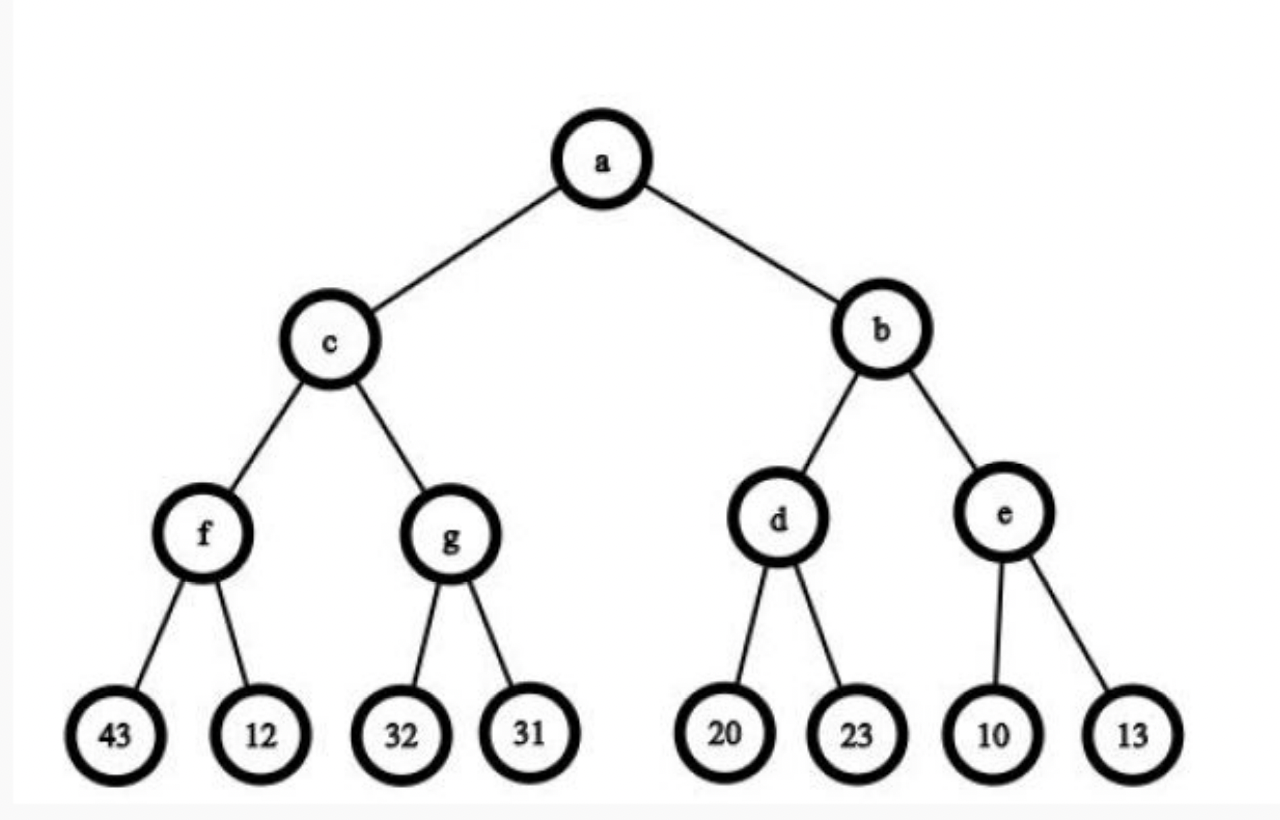
\includegraphics[width=0.8\linewidth]{hw2-figure1.png}
  \caption{第三题的对抗搜索树}
  \label{hw2-figure1}
\end{figure}
    \end{problem}

    \begin{solution}
        \begin{enumerate}
            \item a 为 32,如图 \ref{fig:p301} 所示。
            \begin{figure}[H]
                \centering
                \usetikzlibrary{shapes.geometric}
\begin{tikzpicture}[every node/.style={scale=0.5}]
\tikzstyle{treenode}=[draw,regular polygon, regular polygon sides=3,shape border uses incircle];
\tikzstyle{maxnode}=[treenode];
\tikzstyle{minnode}=[treenode,shape border rotate=60];
\node [maxnode] (v1) at (-0.5,2) {32};
\node [minnode] (v2) at (-2.5,1) {32};
\node [minnode] (v9) at (1.5,1) {13};
\node [maxnode] (v3) at (-3.5,0) {43};
\node [maxnode] (v4) at (-1.5,0) {32};
\node [maxnode] (v10) at (0.5,0) {23};
\node [maxnode] (v11) at (2.5,0) {13};
\node [minnode] (v5) at (-4,-1) {43};
\node [minnode] (v6) at (-3,-1) {12};
\node [minnode] (v7) at (-2,-1) {32};
\node [minnode] (v8) at (-1,-1) {31};
\node [minnode] (v12) at (0,-1) {20};
\node [minnode] (v13) at (1,-1) {23};
\node [minnode] (v14) at (2,-1) {10};
\node [minnode] (v15) at (3,-1) {13};
\draw  (v1) edge (v2);
\draw  (v2) edge (v3);
\draw  (v2) edge (v4);
\draw  (v3) edge (v5);
\draw  (v3) edge (v6);
\draw  (v4) edge (v7);
\draw  (v4) edge (v8);
\draw  (v1) edge (v9);
\draw  (v9) edge (v10);
\draw  (v9) edge (v11);
\draw  (v10) edge (v12);
\draw  (v10) edge (v13);
\draw  (v11) edge (v14);
\draw  (v11) edge (v15);
\node  at (-5,2) {max};
\node at (-5,1) {min};
\node at (-5,0) {max};
\node at (-5,-1) {min};
\end{tikzpicture}
                \caption{题目3第(1)题}\label{fig:p301}
            \end{figure}
            \item 访问了 11 个节点。
            
            \begin{tabular}{l}
                \toprule
                a - c - f - 43 \\
                a - c - f - 12 \\
                a - c - g - 32 \\
                a - c - g - 31 \\
                a - b - d - 20 \\
                a - b - d - 23 \\
                \bottomrule
            \end{tabular}
        \end{enumerate}
    \end{solution}

    \begin{problem}
        \indent 考虑一个这样的CSP问题:我们需要给变量\textit{$X_1, X_2, X_3, X_4$}赋值,需要满足以下约束:$(a)X_1\geq X_2, (b)X_2>X_3\ or\  X_3-X_2=2, (c)X_3\neq X_4, (d)X_1\neq X_3$。

\begin{figure}[H]
  \centering
  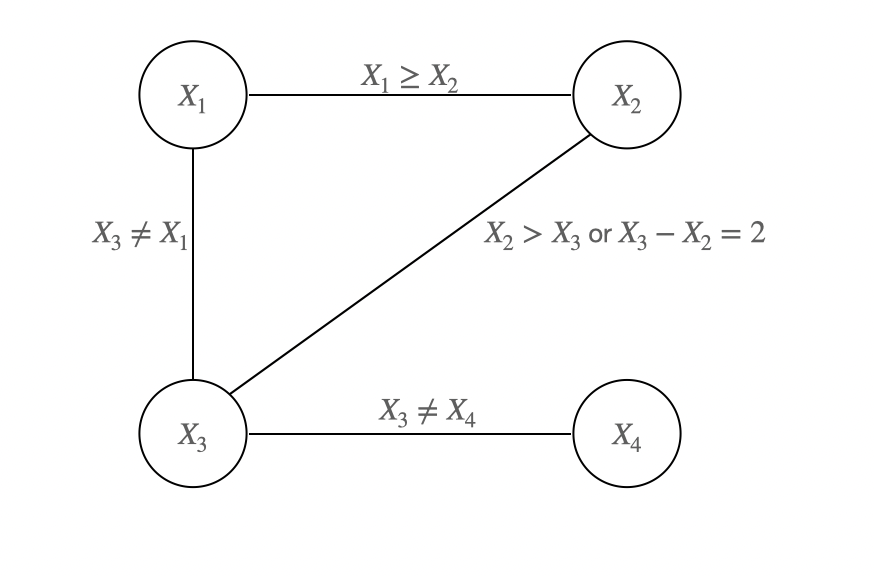
\includegraphics[width=0.5\linewidth]{hw2-figure2.png}
  \caption{第四题的csp问题}
  \label{hw2-figure2}
\end{figure}

\begin{enumerate}
    \item 根据CSP问题赋值求解的Most constraining variable规则,我们应该最先尝试给哪个变量赋值?
    \item 假如我们规定变量变量\textit{$X_1, X_2, X_3, X_4$}的值域分别为$D_1=\{1,2,3,4\}, D_2=\{3,4,5,8,9\}, D_3=\{2,3,5,6,7,9\}, D_4=\{3,5,7,8,9\}$。请问变量\textit{$X_1, X_2, X_3, X_4$}的哪些弧满足弧相容性(arc consistency)?
    \item 我们对该CSP问题在当前状态下运行AC3算法,请完成下方表格的步骤1-7。
\end{enumerate}

\begin{center}
初始的搜索列:$\{ X_2\rightarrow X_1$, $X_1\rightarrow X_2$, $X_3\rightarrow X_2$, $X_2\rightarrow X_3$, $X_4\rightarrow X_3$, $X_3\rightarrow X_4$, $X_3\rightarrow X_1$, $X_1\rightarrow X_3 \}$。\\
\begin{tabular}{|c|c|c|c|}
    \hline 
     步骤& 需要检查的弧$X_i\rightarrow X_j$ & $X_i$值域的变化 & 添加进入搜索列的弧   \\
     \hline 
     0 & $X_2\rightarrow X_1$ & &  \\ \hline
     1 & $X_1\rightarrow X_2$ &  & \\ \hline
     2 & $X_3\rightarrow X_2$ &   &   \\ \hline
     3 & $X_2\rightarrow X_3$ &   &  \\ \hline
     4 & $X_4\rightarrow X_3$ &   &  \\ \hline
     5 & $X_3\rightarrow X_4$ &   &  \\ \hline
     6 & $X_3\rightarrow X_1$ &   &  \\ \hline
     7 & $X_1\rightarrow X_3$ &   & \\ \hline
     ...& ... & ... & \qquad \qquad \qquad \quad ... \\ \hline
\end{tabular}\\
\end{center}
    \end{problem}

    \begin{solution}
        \begin{enumerate}
            \item $X_3$
            % \item $(X_1,X_3),(X_3,X_1),(X_2,X_3),(X_3,X_4),(X_4,X_3)$
            \item $X_3\rightarrow X_1$,$X_1\rightarrow X_3$,$X_2\rightarrow X_3$,$X_4\rightarrow X_3$,$X_3\rightarrow X_4$
            \item 
            % $X\rightarrow Y\Leftrightarrow \forall x\in X \exists y \in Y$
            \begin{center}
                初始的搜索列:$\{ X_2\rightarrow X_1$, $X_1\rightarrow X_2$, $X_3\rightarrow X_2$, $X_2\rightarrow X_3$, $X_4\rightarrow X_3$, $X_3\rightarrow X_4$, $X_3\rightarrow X_1$, $X_1\rightarrow X_3 \}$。\\
                \begin{tabular}{|c|c|c|c|}
                    \hline 
                     步骤& 需要检查的弧$X_i\rightarrow X_j$ & $X_i$值域的变化 & 添加进入搜索列的弧   \\
                     \hline 
                     0 & $X_2\rightarrow X_1$ & $X_2=\{3,4\}$  & 无(因为已经都加入了) \\ \hline
                     1 & $X_1\rightarrow X_2$ & $X_1=\{3,4\}$ & $X_2\rightarrow X_1$ \\ \hline
                     2 & $X_3\rightarrow X_2$ & $X_3=\{2,3,5,6\}$  & 无  \\ \hline
                     3 & $X_2\rightarrow X_3$ & 无变化 & 无 \\ \hline
                     4 & $X_4\rightarrow X_3$ &  无变化 & 无 \\ \hline
                     5 & $X_3\rightarrow X_4$ &  无变化 & 无 \\ \hline
                     6 & $X_3\rightarrow X_1$ &  无变化 & 无 \\ \hline
                     7 & $X_1\rightarrow X_3$ & 无变化  & 无 \\ \hline
                     ...& ... & ... & \qquad \qquad \qquad \quad ... \\ \hline
                \end{tabular}\\
                \end{center}
        \end{enumerate}
    \end{solution}

\end{document}